\chapter{Introduzione}

La gestione dinamica della memoria è una delle principali responsabilità dei sistemi operativi moderni\footnotemark. Essa ospita i processi attivi e i dati correntemente elaborati dal software in esecuzione; in quanto più veloce da accedere dei dispositivi di memoria di massa, spesso viene usata come intermediario nella comunicazione tra questi ultimi e i processi. Con l'avvento dei sistemi multiprogrammati, la suddivisione della memoria in partizioni dedicate a ogni \textit{task} è diventata un aspetto principale dell'attività dei sistemi operativi: partizionare la memoria in aree contingentate rapidamente e efficacemente è un compito sfidante. 

\begin{quote}
“Memory is the new disk and disk is the new tape.”\\
\hfill --- Jim Gray
\end{quote}

\footnotetext{Dove per memoria si intende la \textit{Random Access Memory}, o RAM.}

Il sistema operativo si deve occupare di gestire e monitorare lo stato di ciascun indirizzo di memoria fisica, regolando l'allocazione della memoria tra i processi concorrenti, e definire le politiche di assegnazione, stabilendo le modalità di accesso alla memoria e le quantità disponibili per ciascun entità. Durante l'allocazione, il sistema operativo determina gli indirizzi di memoria da assegnare e ne mantiene traccia, aggiornandone lo stato in caso di rilascio (deallocazione). Un ulteriore aspetto che richiede attenzione è la memoria di cui il sistema operativo stesso ha necessità per svolgere le sue funzioni; poiché esso adempie a numerosi compiti, laddove le strutture in atto per gestire le sue necessità siano lente o abbiamo un grande sovracosto ciò potrebbe portare a risultati disastrosi per la generale fluidità del calcolatore.

Quando la grandezza del programma è nota alla compilazione e non cambia, è semplice segnalare al sistema operativo quanta memoria sarà necessaria per tutto il ciclo di vita. Questa memoria viene chiamata \textbf{staticamente allocata}. L'incarico di gestione in questo caso risulta dunque semplificato: tuttavia, non sempre è possibile determinare a priori le necessità del programma, in quanto queste potrebbero dipendere da vari fattori che non sono noti al programmatore (e.g. \textit{user input}). Un primo approccio, semplice ma dispendioso, consiste nell'allocare staticamente la memoria necessaria nel \textit{worst case scenario}, ossia prevedere in anticipo quale possa essere il bisogno di memoria più elevato nel corso della vita del programma e richiedere questa quantità. In questo modo però la memoria disponibile per il sistema operativo potrebbe risultare nulla\footnotemark quando invece i processi impediscono l'uso di \textit{working storage} non utilizzato al momento ed esistono casi per cui svolgere questo calcolo è impossibile, poiché il tetto massimo è imprevedibile. In generale questa pratica risulta inapplicabile in contesti dove la quantità di memoria non è abbondante.

\footnotetext{Out of memory (OOM) error}

L'alternativa giunge immediata, ma non di facile implementazione: fornire al programmatore sistemi per \textbf{allocare dinamicamente} la memoria, ossia per variare la grandezza dell'area dedicata ai dati del programma durante la sua vita, ingrandendola e restringendola in base alle necessità. In questo modo, le risorse sono occupate solamente quando sono necessarie e nel momento in cui non sono più utili vengono restituite al sistema operativo, che le può concedere a un altro richiedente. Il processo di allocazione consiste dunque nel gestire efficacemente la condivisione del \textit{dynamic storage} tra vari programmi, rispondendo alle loro richieste in modo appropriato. Affinché ciò avvenga, si attinge a un'area contigua denominata \textit{heap} (o \textit{free store}). 

\begin{figure}[H]
  \centering
  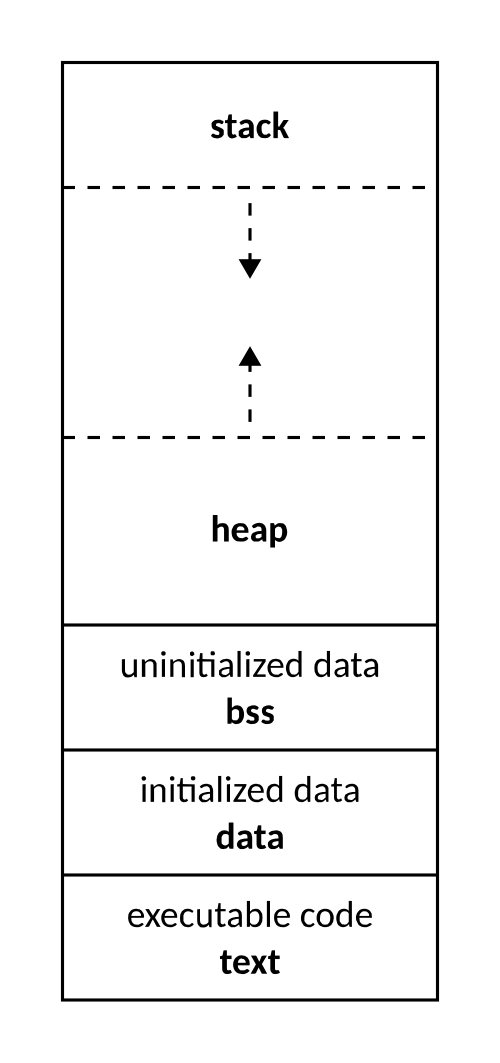
\includegraphics[width=0.2\textwidth]{images/program_memory_layout.png}
  \caption{Layout semplificato della memoria di un programma.}
  \label{fig:program_memory_layout}
\end{figure}

\paragraph{Memoria dinamica a user level.} 
Generalmente, quando facciamo riferimento alla gestione di memoria, parliamo di una componente del sistema operativo, che ha dunque privilegi diversi e un grado maggiore di autonomia rispetto a un programma in esecuzione. Tuttavia, questa operazione va svolta anche nei casi \textit{bare metal}, dove \textbf{non esiste un mediatore della comunicazione tra i programmi utente e le risorse}; allo stesso modo non è irragionevole pensare che amministrare autonomamente la memoria possa essere utile all'utente in determinati contesti. Ad esempio, in applicazioni \textit{embedded} o \textit{real-time}, dove è fondamentale garantire tempi di risposta prevedibili, può un approccio personalizzato al problema migliorare le prestazioni? In altri casi, come nei database o in sistemi \textit{high performance}, tecniche specializzate possono ottimizzare l'uso della memoria, migliorando determinate metriche obiettivo. Nel corso del progetto, particolare attenzione è stata posta nel sottolineare in quali situazioni sia più vantaggioso un determinato approccio piuttosto che affidarsi a una soluzione generica.

\section{\textit{Memory Allocators}}

In un dato istante, alcune regioni dell'\textit{heap} sono riservate (in uso da parte di processi o strutture dati), mentre altre rimangono libere (non allocate) e pertanto disponibili per esaudire future richieste. \textbf{Il \textit{Memory Allocator} è il modulo specializzato del sistema operativo che sovrintende all'assegnazione e al rilascio della memoria}. All'inizializzazione gli viene assegnata per il suo uso una quantità di byte; esso si occupa dunque di gestirli dinamicamente. Ciò può avvenire secondo strategie e politiche ben diverse: obiettivo di questo progetto è l'esplorazione di un sottoinsieme rappresentativo di questi moduli, caratterizzati da un campione delle suddette strategie, evidenziando nelle loro implementazioni i benefici e i punti deboli.

Il programma dell'utente manipola o muta lo stato della memoria. L'allocatore non ha alcuna informazione sulle operazioni svolte dai processi e sul contenuto della RAM e, una volta assegnata della memoria, deve rispettare le indicazioni dell'utente: non può pertanto sottrarre la risorsa per riorganizzarsi. In altre parole, l'algoritmo di assegnazione è \textit{online} (possiede informazioni limitate) e \textit{real-time} (ha dei vincoli sul tempo per rispondere). Svolge delle valutazioni seguendo euristiche di comportamento: nei capitoli successivi verranno analizzate in dettaglio alcune di esse, con particolare attenzione alle loro implementazioni pratiche e ai contesti applicativi in cui risultano più efficaci. 

\paragraph{Allocazione manuale o automatica della memoria.}
Linguaggi di programmazione diversi gestiscono questa problematica secondo principalmente due paradigmi: l'allocatore può funzionare in modo manuale, ossia rispondendo alla chiamata esplicita di funzioni che comunicano le necessità del programma, o in modo automatico, attraverso un ulteriore modulo che prende il nome di \textit{garbage collector}. Quest'ultimo consiste in un insieme di \textit{routine} che determinano se esiste memoria che sia irraggiungibile dal programma, in quanto ogni riferimento ad essa sia stato perso. Quest'ultima viene riconsegnata all'allocatore per esaudire richieste future. Esistono diversi meccanismi per effettuare questa analisi, ma nel corso della nostre riflessioni ci concentreremo sull'allocazione manuale di memoria, in particolare nelle modalità in cui avviene nel linguaggio di programmazione \textbf{C}. 

\section{Svolgimento del progetto}
L'obiettivo di questo progetto è duplice: da una parte vedremo i benefici che possono essere ricavati dalla scelta delle corrette strategie in base alle necessità dell'applicazione, senza affidarsi a soluzioni generiche; dall'altra illustreremo le opportunità che sono fornite dallo studio del comportamento dei propri programmi. Gli sviluppatori avveduti possono usare a qesto scopo strumenti preesistenti o di propria creazione. Nessuno può conoscere le esigenze di gestione dinamica della memoria di un programma come il suo creatore e, per quanto le euristiche adoperate possano essere brillanti in assenza di dati più specifici, è appropriato che egli compia scelte ragionate e, laddove sia necessario, implementi una soluzione \textit{ad hoc} piuttosto che affidarsi a un sistema inadatto.

Nel secondo capitolo, esploriamo la letteratura accademica alla base delle scelte progettuali, senza scendere nel dettaglio su specifiche implementazioni degli algoritmi di \textit{allocation}, ma acquistando una visuale storica e contestuale sull'argomento. Approfondiamo le motivazioni per cui esistono riserve e preoccupazioni sull'assegnazione dinamica in determinate applicazioni e, citando articoli rilevanti, stabiliamo le basi formali per le valutazioni del lavoro svolto. Forniamo quindi risorse utili per acquisire informazioni sull'argomento anche per chi si trovi ad affrontarlo per la prima volta e menzioniamo le opere che sono state d'ispirazione. 

In seguito descriviamo i gestori di memoria sviluppati nel corso del progetto: lo \texttt{SlabAllocator}, il \texttt{BuddyAllocator} e il \texttt{BitmapBuddyAllocator}. Analizziamo le tecniche adoperate e giustifichiamo le scelte implementative prese nel contesto didattico del corso di Sistemi Operativi. Esplicitiamo dunque quali siamo le metriche d'interesse per valutare la performance degli allocatori: stabiliamo contemporaneamente le nostre aspettative riguardo i risultati che ci aspettiamo di riscontrare.

Nel capitolo successivo, infatti, ci occupiamo dapprima di valutare la correttezza dei risultati ottenuti, attraverso una serie di test che ci forniscano la certezza che gli allocatori si comportino come desiderato, e in secondo luogo poniamo le basi per un analisi più approfondita creando un linguaggio che possiamo adoperare per descrivere formalmente un \textit{benchmark}: l'unico modo infatti di poter fare una scelta consapevole è riflettere attentamente sull'efficienza delle soluzioni adottate e indagare a fondo i procedimenti per acquisire un'intuizione dei costi e dei \textit{trade-off}.
Una volta fatto ciò, osserviamo i risultati e li confrontiamo con le ipotesi fatte durante la descrizione dell'implementazione, valutando il comportamento e cercando di spiegare eventuali fenomeni imprevisti. 